\documentclass{article}

\usepackage[utf8]{inputenc}
\usepackage{setspace}
\usepackage[
	a4paper,
	total={17cm,25cm},
	top=3cm, left=2cm,
	includefoot
	]{geometry}
\usepackage[
	english,
	czech
	]{babel}
\usepackage[autostyle]{csquotes}
\usepackage{caption}
\usepackage{graphicx}
\graphicspath{{./assets/}}

\title{Návrh hry - Blokranč}
\author{Petr Maronek}
\date{5.11.2022}

% 	Vysvětlivky
%	\section* hvězdička znamená, že má LaTeX odebrat číslování

\begin{document}
	\begin{spacing}{1.15}
		\rmfamily
		\maketitle
		\begin{center}
			\textbf{Vysoká škola finanční a správní}\linebreak
			Návrh počítačových her\linebreak
			Zimní semestr 2022\linebreak
			Vedoucí práce: \textbf{doc. Ing Stanislava Mildeová CSc.}
		\end{center}
		\pagebreak
			
		\section*{Abstrakt}
		Hra v prohlížeči na bázi těžby herních prostředků, která umožňuje hráči reálně zhodnocovat své majetky v herním prostředí. Pomocí herních tokenů může zdokonalovat své NFT nástroje, které těží více těchto tokenů. Tokeny a NFT se poté dají prodat na trhu za reálnou hodnotu.
				
		\section*{Klíčová slova}
		krypto, NFT, farma, playToEarn, prohlížeč
		\pagebreak
		    
		\section*{Úvod}
		Hra je postavená na \textbf{blockchain} technologii. Níže je zobrazena myšlenková mapa, která zobrazuje prvky hry.\linebreak
		
		\label{Myšlenková mapa}
		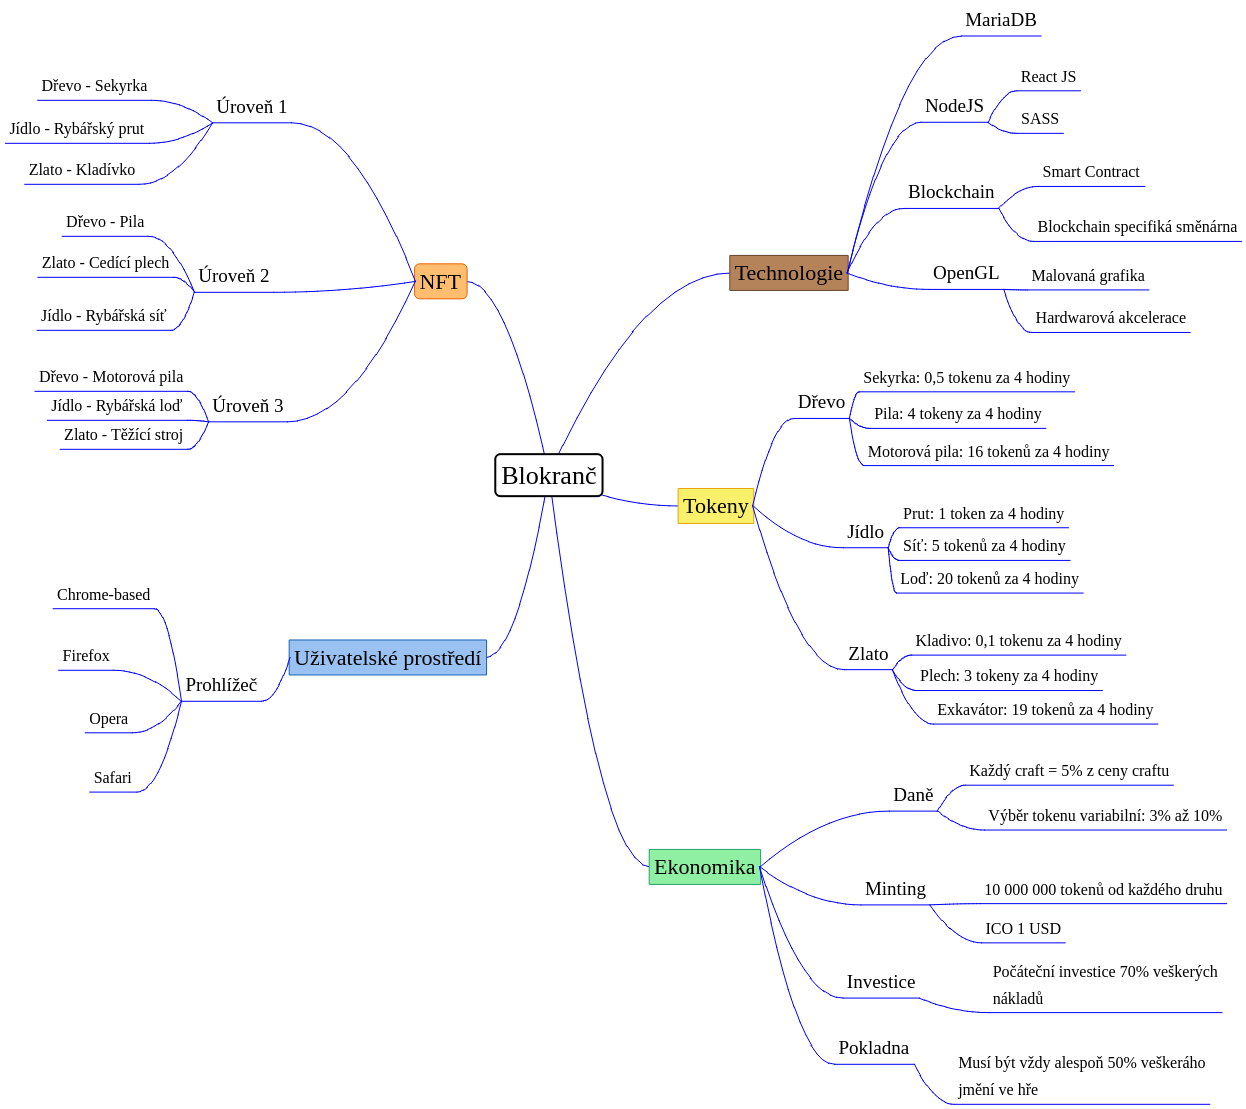
\includegraphics[scale=0.3]{221104-NPH-Blokranč.png}
		\captionof{figure}{Myšlenková mapa}
		
		A pokračujeme v textu dál.
	
	\end{spacing}
\end{document}

